\section{Resultados}


\subsection{Diseño de Interfaces y Mockups}

Antes de comenzar a programar el sistema SAGAI, se diseñaron las pantallas y la experiencia de usuario utilizando Figma. Hacer esto primero fue de mucha ayuda para organizar dónde iban a estar acomodados los botones, las tablas y los formularios, asegurando que la navegación fuera sencilla e intuitiva para los usuarios.

Como se puede ver en la Figura \ref{fig:figma_flujo}, se armó un prototipo donde se conectaron las distintas vistas del sistema. Esto sirvió para simular cómo funcionaría el paso desde el directorio de expedientes hacia las ventanas emergentes (modales) de captura, y finalmente hacia la pantalla donde trabaja la Inteligencia Artificial.

\begin{figure}[H]
    \centering
    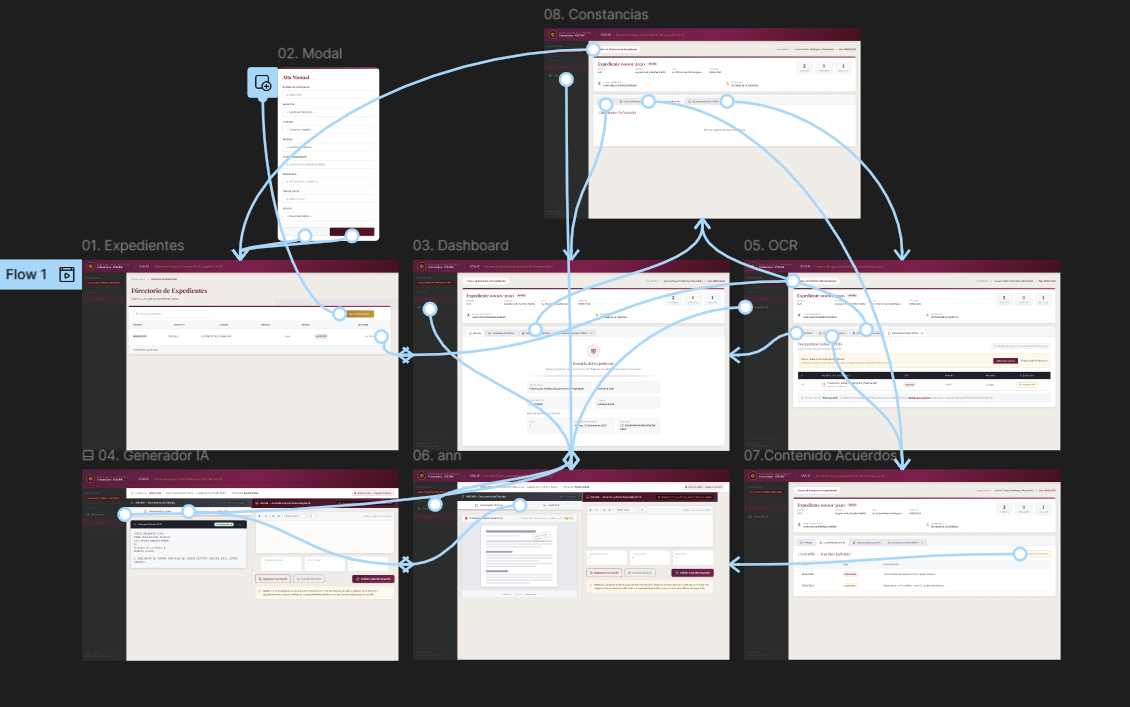
\includegraphics[width=0.9\textwidth]{img/figma_conexiones.png}
    \caption{Diseño de las pantallas y conexiones del sistema elaborado en Figma.}
    \label{fig:figma_flujo}
\end{figure}

\textbf{Nota:} Si se está revisando este documento en formato digital, se puede probar la navegación del diseño haciendo clic en el siguiente enlace: \href{https://www.figma.com/proto/U4WAHxoMm39aukToa0Pttl/Sin-t%C3%ADtulo?node-id=0-1&t=TPFTQtxiZDvdafTd-1}{Prototipo interactivo de SAGAI en Figma}.

Finalmente, para tener una presentación más realista del diseño, se generaron \textit{mockups} (como el que se muestra en la Figura \ref{fig:mockup_directorio}). Estas imágenes sirven para mostrar exactamente cómo se va a adaptar la interfaz web cuando el personal del juzgado la abra y la trabaje desde sus laptops.

\begin{figure}[H]
    \centering
    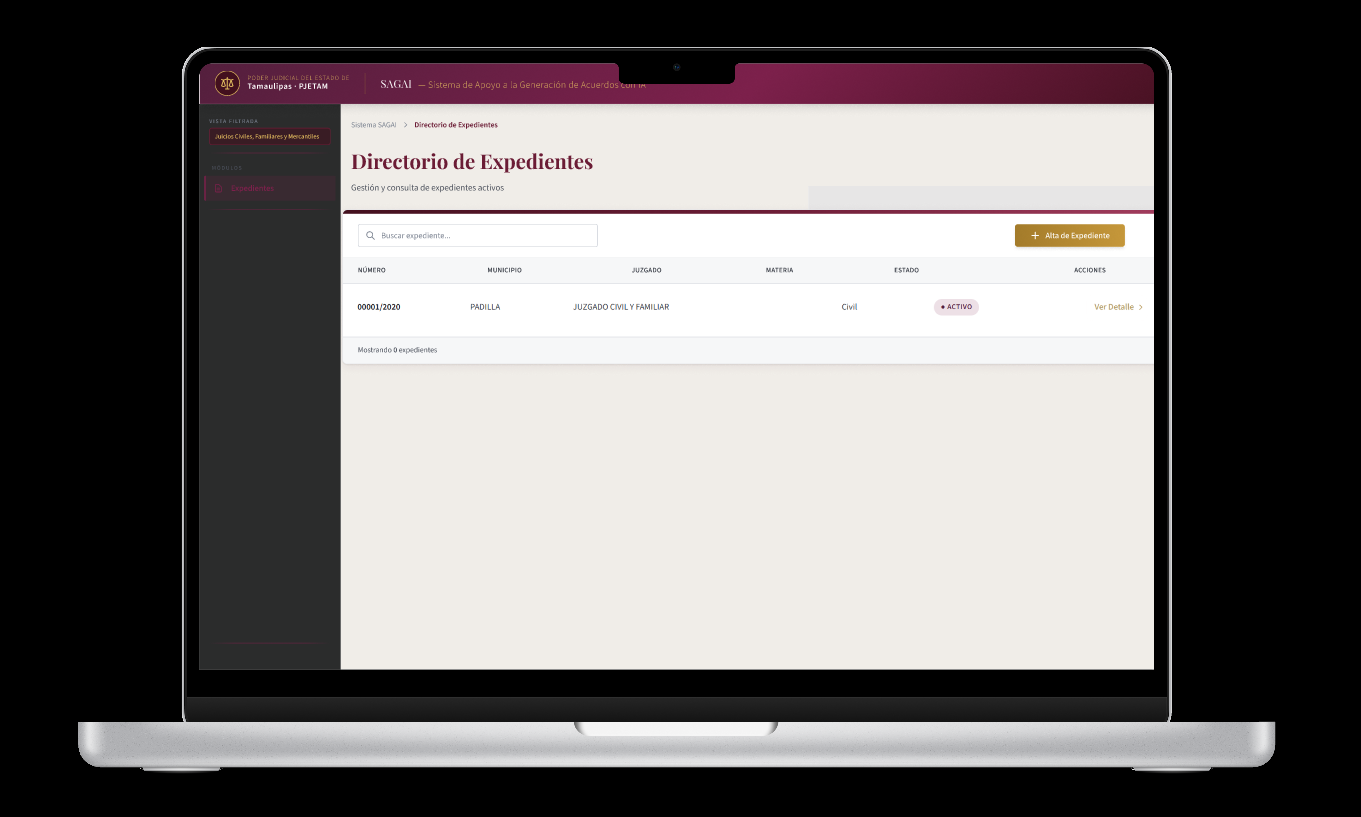
\includegraphics[width=0.9\textwidth]{img/mockup_directorio.png}
    \caption{Mockup de cómo se ve el Directorio de Expedientes en una pantalla de computadora.}
    \label{fig:mockup_directorio}
\end{figure}

\subsection{Desarrollo del Sistema (Frontend e Integración IA)}

Para el desarrollo de SAGAI, el enfoque principal fue crear una interfaz práctica, rápida y fácil de usar para el personal del juzgado. Todo el trabajo visual y de interacción se concentró en el Frontend, utilizando tecnologías web actuales para asegurar que el sistema funcionara sin problemas.

\subsubsection{Construcción del Frontend}
Las pantallas del sistema se maquetaron utilizando HTML5 para organizar bien la información, mientras que los estilos y el diseño visual se trabajaron con CSS3 puro. Esto garantizó que el sistema se viera bien y fuera compatible con los navegadores de las computadoras del tribunal.

Para darle vida a la interfaz y hacerla interactiva, se utilizó JavaScript puro (Vanilla JS). Al no depender de librerías externas pesadas, el sistema carga mucho más rápido. Algunas de las cosas más importantes que se programaron incluyen:
\begin{itemize}
    \item \textbf{Uso de Modales:} En lugar de mandar al usuario a otra página cada vez que necesita registrar algo (como en el alta de expedientes), se programaron ventanas emergentes. Así, la navegación es mucho más fluida y el usuario no pierde de vista lo que estaba haciendo.
    \item \textbf{Peticiones Asíncronas (Fetch API):} Se escribieron funciones para que el Frontend se pudiera comunicar con el servidor en segundo plano. Esto permite guardar y consultar datos en formato JSON sin tener que estar recargando la página a cada rato.
    \item \textbf{Manejo de Respuestas de la IA:} Se creó la lógica necesaria para recibir el texto generado por la Inteligencia Artificial y colocarlo directamente en un editor dentro de la pantalla, para que el secretario de acuerdos pueda revisarlo y editarlo al momento.
\end{itemize}

\subsubsection{Integración de la Inteligencia Artificial (API de Claude)}
Una parte clave del proyecto fue conectar el sistema con Claude, el modelo de inteligencia artificial de Anthropic. Esta conexión se hizo mediante su API REST, lo que nos permite enviarle el texto del documento original (obtenido por el OCR) y recibir de vuelta una propuesta de acuerdo judicial.

Para que esto funcionara correctamente en el sistema, se trabajó en lo siguiente:
\begin{enumerate}
    \item \textbf{Diseño de Prompts:} Se configuraron instrucciones muy precisas para la IA, indicándole que debía comportarse como un asistente legal y basarse en el Código de Procedimientos Civiles de Tamaulipas para redactar los acuerdos, usando únicamente la información del expediente.
    \item \textbf{Ajuste de Parámetros:} Se modificaron algunas opciones en la API (como \textit{max\_tokens} y \textit{temperature}) para asegurar que las respuestas fueran formales, precisas y no tardaran demasiado en mostrarse en la pantalla.
    \item \textbf{Seguridad desde el Backend:} Para que las claves de la API estuvieran seguras, las peticiones a Claude no se hacen directo desde el navegador, sino que pasan por el servidor de FastAPI, el cual procesa la información antes de mandarla a la pantalla del usuario.
\end{enumerate}

Al final, se logró que la inteligencia artificial se sintiera como una herramienta natural dentro del sistema, funcionando como un apoyo rápido que siempre deja la decisión final y la revisión en manos del personal humano.


\subsection{Modelado del Sistema}

Para tener una visión clara de cómo funciona SAGAI por dentro, cómo se estructura su información y cómo interactúan los usuarios con él, se elaboraron los siguientes diagramas. Estos modelos fueron fundamentales para guiar la programación del sistema.

\subsubsection{Diagrama de Casos de Uso}
Este diagrama nos ayuda a identificar rápidamente quiénes son los actores que interactúan con el sistema (por ejemplo, el Secretario de Acuerdos) y cuáles son las acciones principales que pueden realizar, como dar de alta expedientes, subir documentos o generar un acuerdo usando la Inteligencia Artificial.

\begin{figure}[H]
    \centering
    \includegraphics[width=0.55\textwidth]{img/Caso_uso.pdf}
    \caption{Diagrama de Casos de Uso de SAGAI.}
    \label{fig:caso_uso}
\end{figure}

\subsubsection{Diagrama de Base de Datos}
Para el almacenamiento de la información, se diseñó un modelo relacional. En este diagrama (Entidad-Relación) se muestran las tablas principales del sistema, como la de usuarios, expedientes y los documentos generados. Aquí se definen qué datos se guardan y cómo se conectan entre sí para mantener la información del juzgado organizada.

\begin{figure}[H]
    \centering
    \includegraphics[width=0.85\textwidth]{img/DiagramaDER.pdf}
    \caption{Modelo Entidad-Relación de la base de datos.}
    \label{fig:diagrama_bd}
\end{figure}

\subsubsection{Diagrama de Actividades}
Aquí se ilustra el paso a paso o el "flujo de trabajo" que sigue el sistema. Muestra el camino lógico que toma la información desde que el usuario inicia sesión, busca un expediente, procesa un documento con OCR, hasta que finalmente valida y guarda el acuerdo generado por la IA.

\begin{figure}[H]
    \centering
    \includegraphics[width=0.55\textwidth]{img/Diagrama_Actividades.pdf}
    \caption{Diagrama de Actividades del proceso de generación de acuerdos.}
    \label{fig:diagrama_actividades}
\end{figure}

\subsubsection{Diagrama de Secuencia}
Finalmente, este diagrama es clave para entender la comunicación "por detrás" del sistema. Muestra en orden cronológico cómo el Frontend (la interfaz del usuario) hace peticiones al Backend (el servidor en FastAPI), y cómo este último se comunica de forma segura con la API externa de Claude para obtener el texto del acuerdo y regresarlo a la pantalla.

\begin{figure}[H]
    \centering
   
    \includegraphics[width=0.85\textwidth]{img/Diagrama_de_secuencia.pdf}
    \caption{Diagrama de Secuencia de la comunicación entre Frontend, Backend y la API de IA.}
    \label{fig:diagrama_secuencia}
\end{figure}

\subsection{Resultado Final: Pantallas del Sistema}

Después de concluir las fases de diseño y desarrollo, el resultado final es un sistema web completamente funcional, rápido e intuitivo. A continuación, se presenta un recorrido visual por las interfaces principales del sistema, ilustrando el flujo de trabajo real de un usuario desde que ingresa hasta que genera un acuerdo apoyado por Inteligencia Artificial.

\subsubsection{Directorio y Registro de Expedientes}
Al iniciar sesión, la primera pantalla que recibe al usuario es el \textbf{Directorio de Expedientes} (Figura \ref{fig:pantalla_directorio}). Esta es la mesa de trabajo principal, donde se pueden buscar, filtrar y visualizar rápidamente todos los casos que lleva el juzgado. 

Si llega un caso nuevo, el usuario hace clic en el botón de ``Alta de Expediente'', lo cual despliega una ventana emergente o modal (Figura \ref{fig:pantalla_alta}). Esto permite registrar los datos esenciales (municipio, juzgado, materia, actor y demandado) de forma rápida y sin tener que abandonar la vista principal.
\begin{figure}[H]
    \centering
    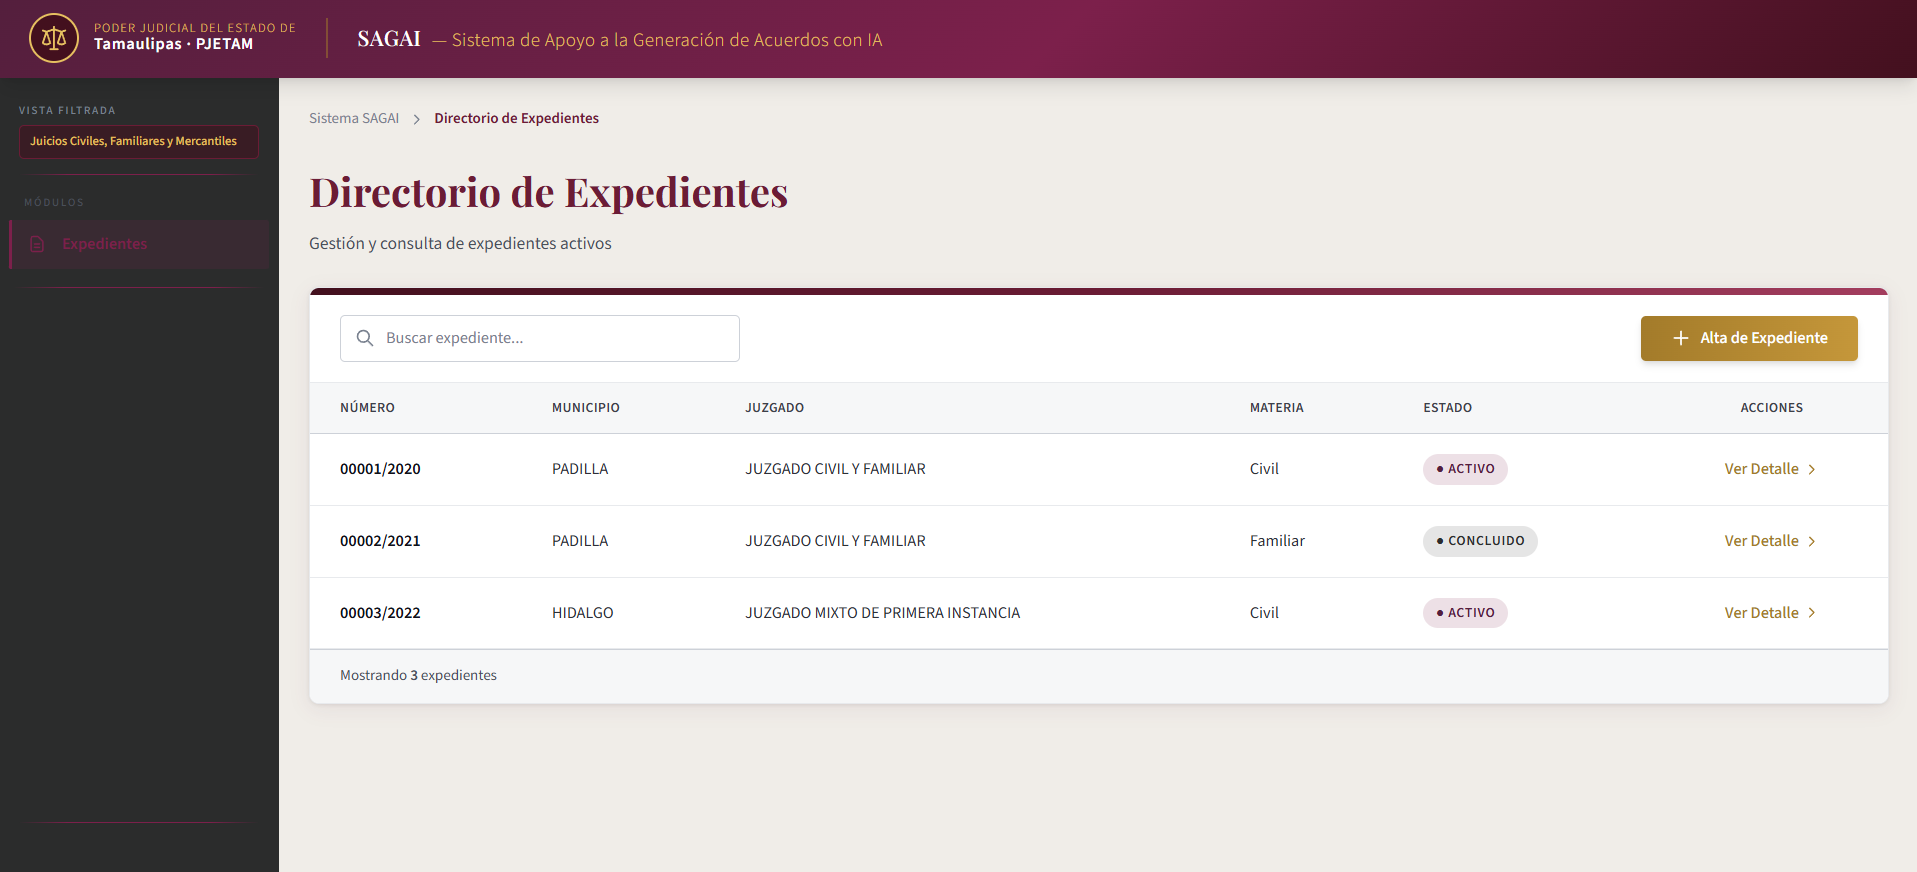
\includegraphics[width=0.9\textwidth]{img/Expedientes.png}
    \caption{Vista principal del Directorio de Expedientes.}
    \label{fig:pantalla_directorio}
\end{figure}

\begin{figure}[H]
    \centering
    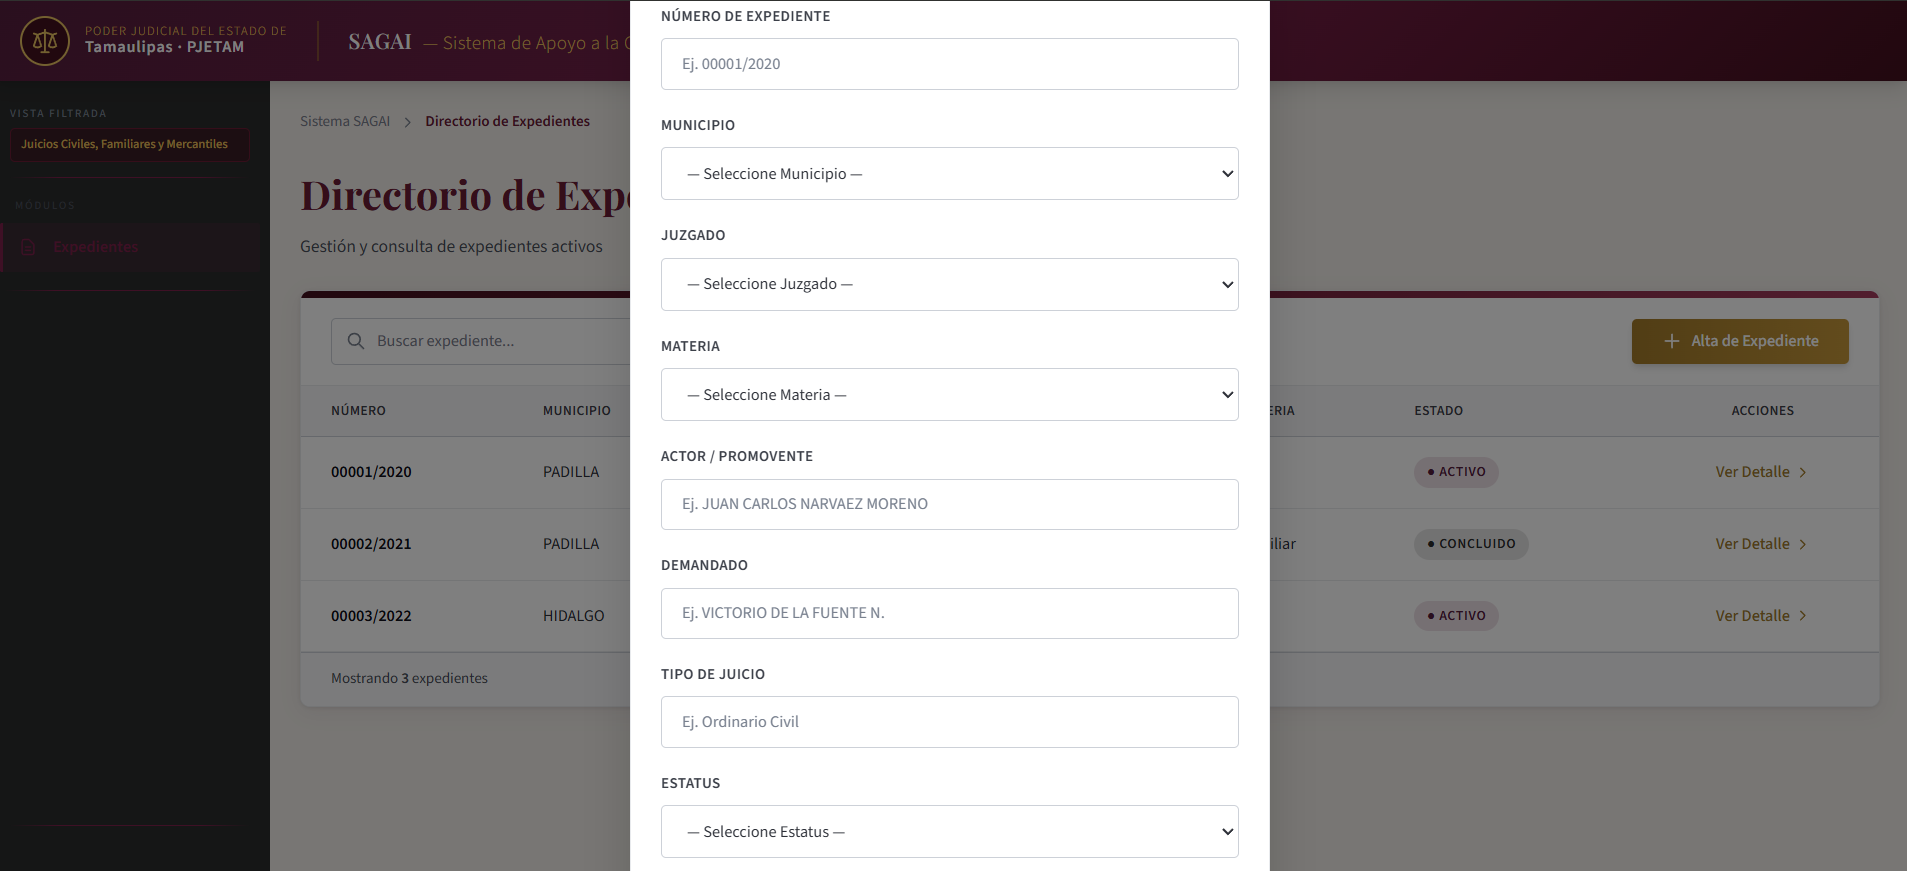
\includegraphics[width=0.6\textwidth]{img/modal_Alta.png}
    \caption{Ventana modal para dar de alta un nuevo expediente.}
    \label{fig:pantalla_alta}
\end{figure}

\subsubsection{Vista General del Expediente y sus Pestañas}
Al seleccionar "Ver Detalle`` en algún caso (por ejemplo, el 00001/2020), el sistema nos lleva al interior del expediente (Figura \ref{fig:pantalla_expediente}). La parte superior siempre muestra un encabezado con los datos clave para que el usuario no pierda el contexto, además de un contador rápido de acuerdos y documentos pendientes.

La navegación interna se divide en pestañas. La primera es la \textbf{Portada} (Figura \ref{fig:pantalla_portada}), que funciona como la carátula física del expediente, mostrando el tipo de juicio, la vía, la etapa procesal y la fecha de presentación original.

\begin{figure}[H]
    \centering
    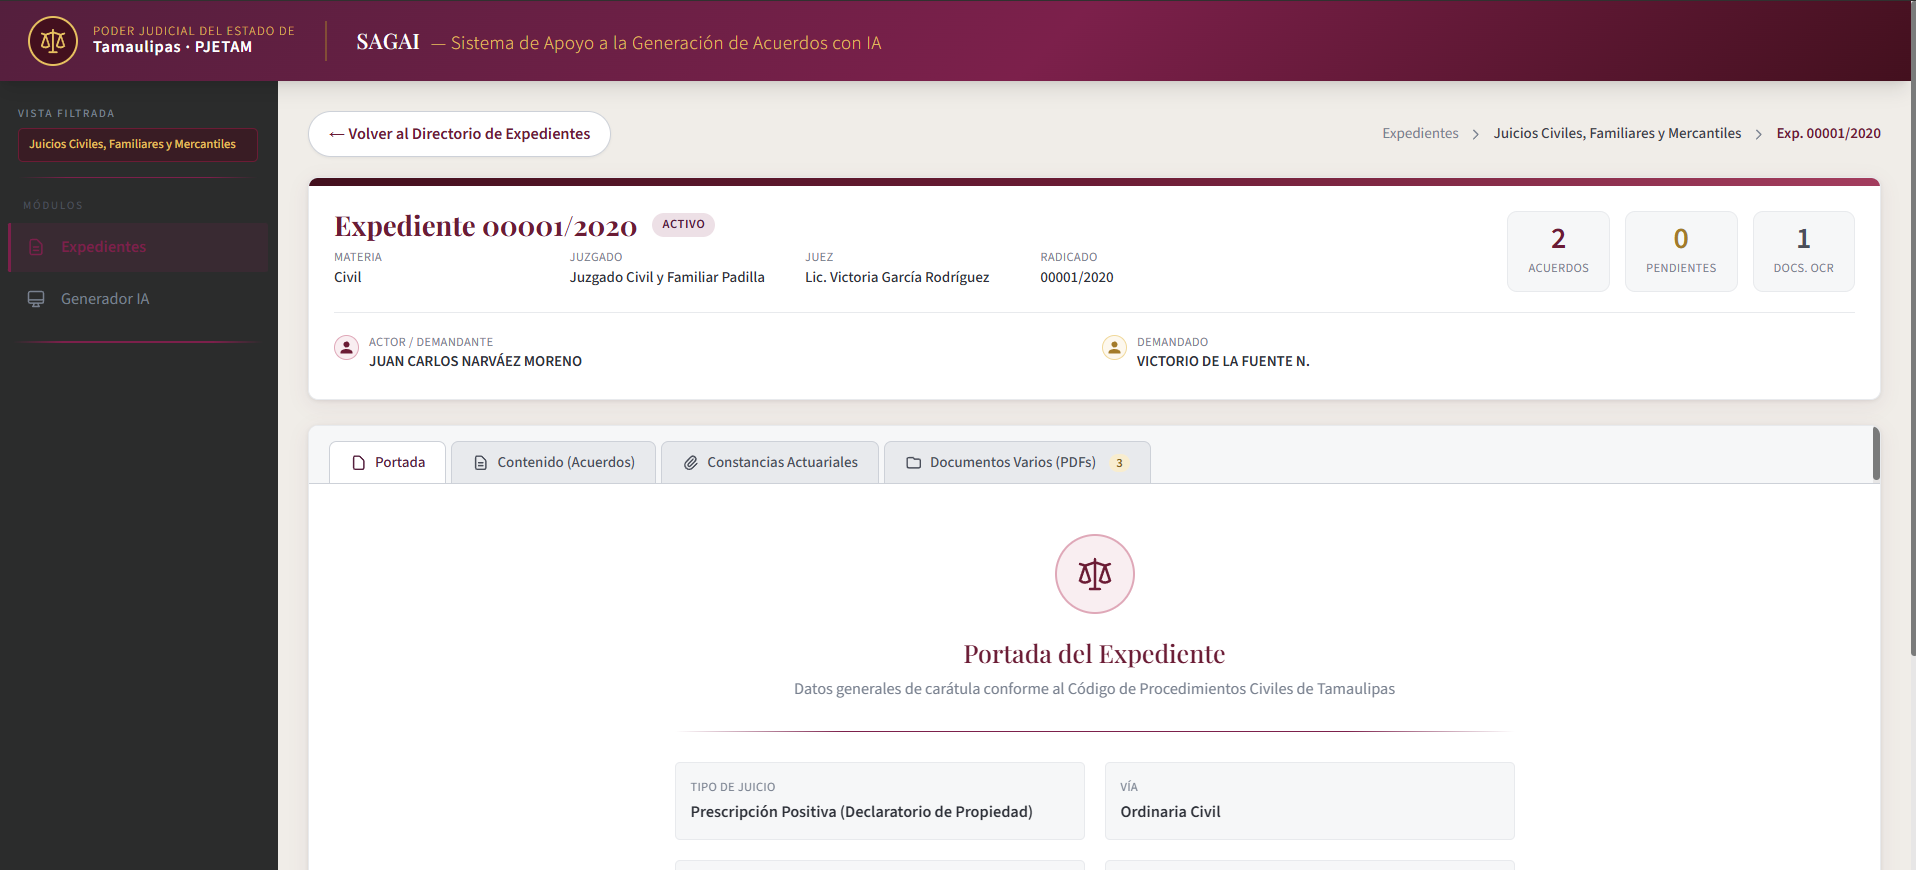
\includegraphics[width=0.9\textwidth]{img/expediente.png}
    \caption{Vista general al ingresar a un expediente específico.}
    \label{fig:pantalla_expediente}
\end{figure}

\begin{figure}[H]
    \centering
    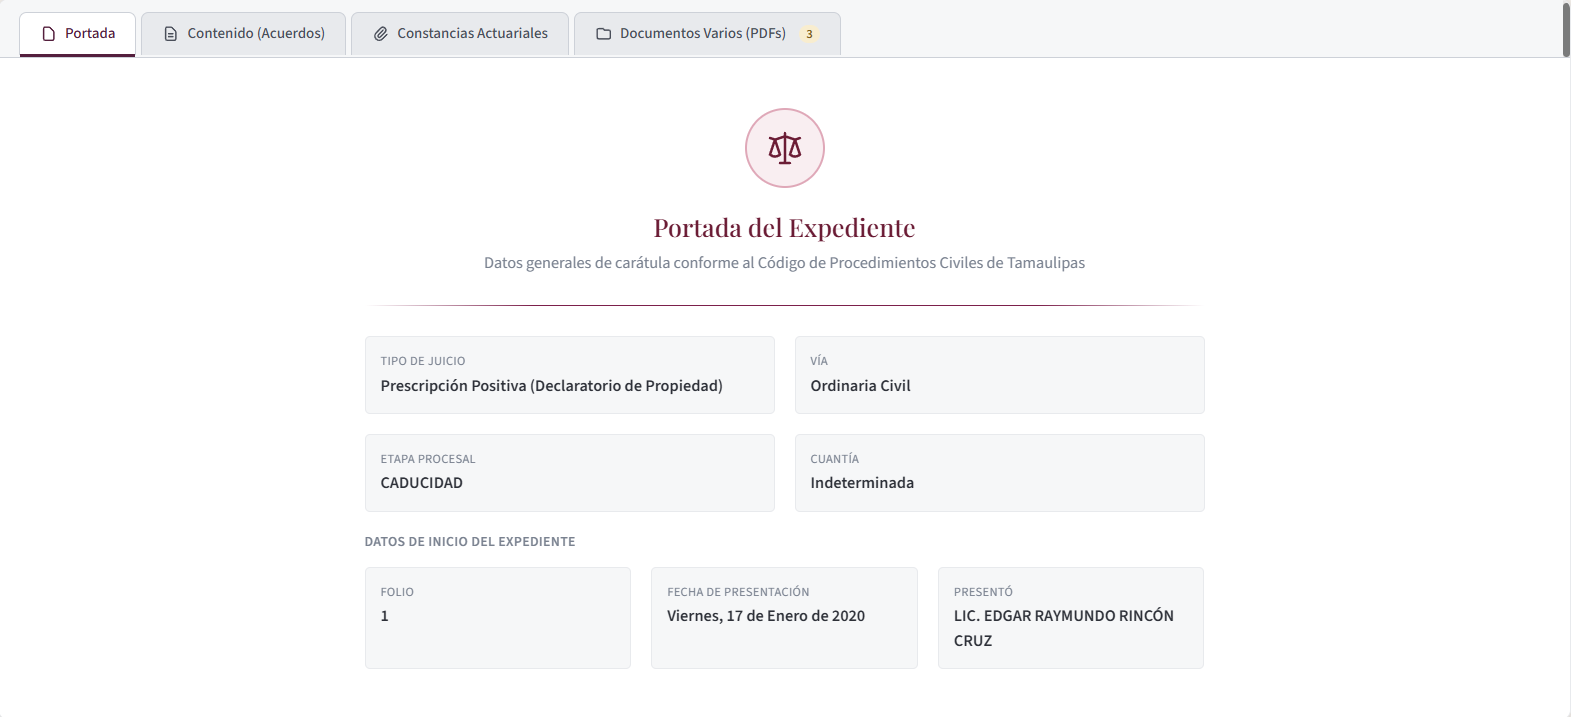
\includegraphics[width=0.9\textwidth]{img/PortadA.png}
    \caption{Pestaña de Portada con el resumen del juicio.}
    \label{fig:pantalla_portada}
\end{figure}

\subsubsection{Historial de Acuerdos y Constancias}
Para mantener el orden cronológico del caso, el sistema cuenta con apartados específicos. La pestaña de \textbf{Contenido (Acuerdos)} (Figura \ref{fig:pantalla_acuerdos}) despliega una lista de todas las resoluciones que ya se han emitido, con su fecha y tipo. Por otro lado, la pestaña de \textbf{Constancias Actuariales} (Figura \ref{fig:pantalla_constancias}) está reservada exclusivamente para los registros de notificaciones, citatorios o diligencias realizadas por el actuario.

\begin{figure}[H]
    \centering
    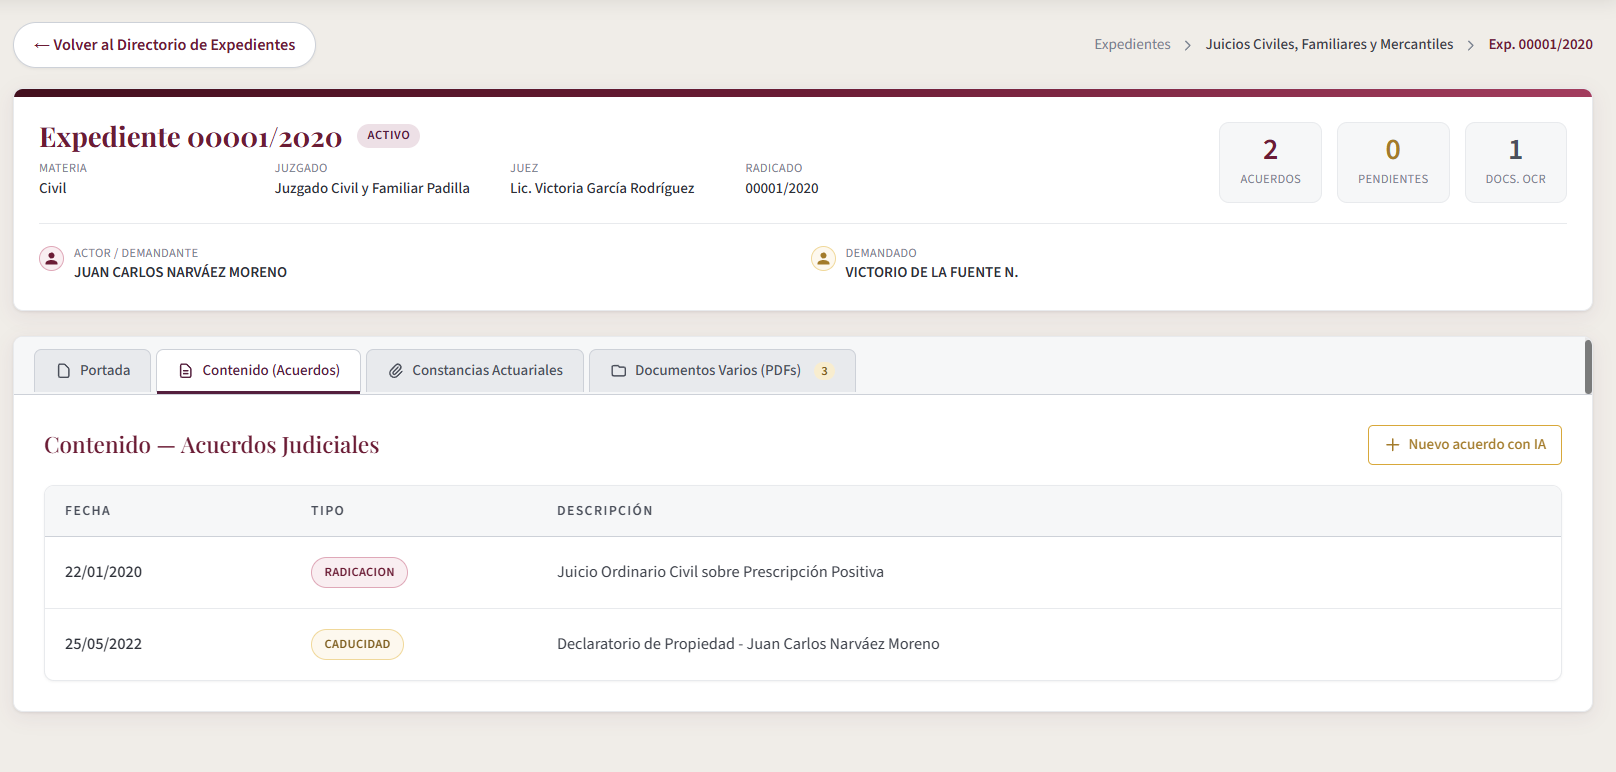
\includegraphics[width=0.9\textwidth]{img/contenido_Acuerdo.png}
    \caption{Historial de acuerdos emitidos dentro del expediente.}
    \label{fig:pantalla_acuerdos}
\end{figure}

\begin{figure}[H]
    \centering
    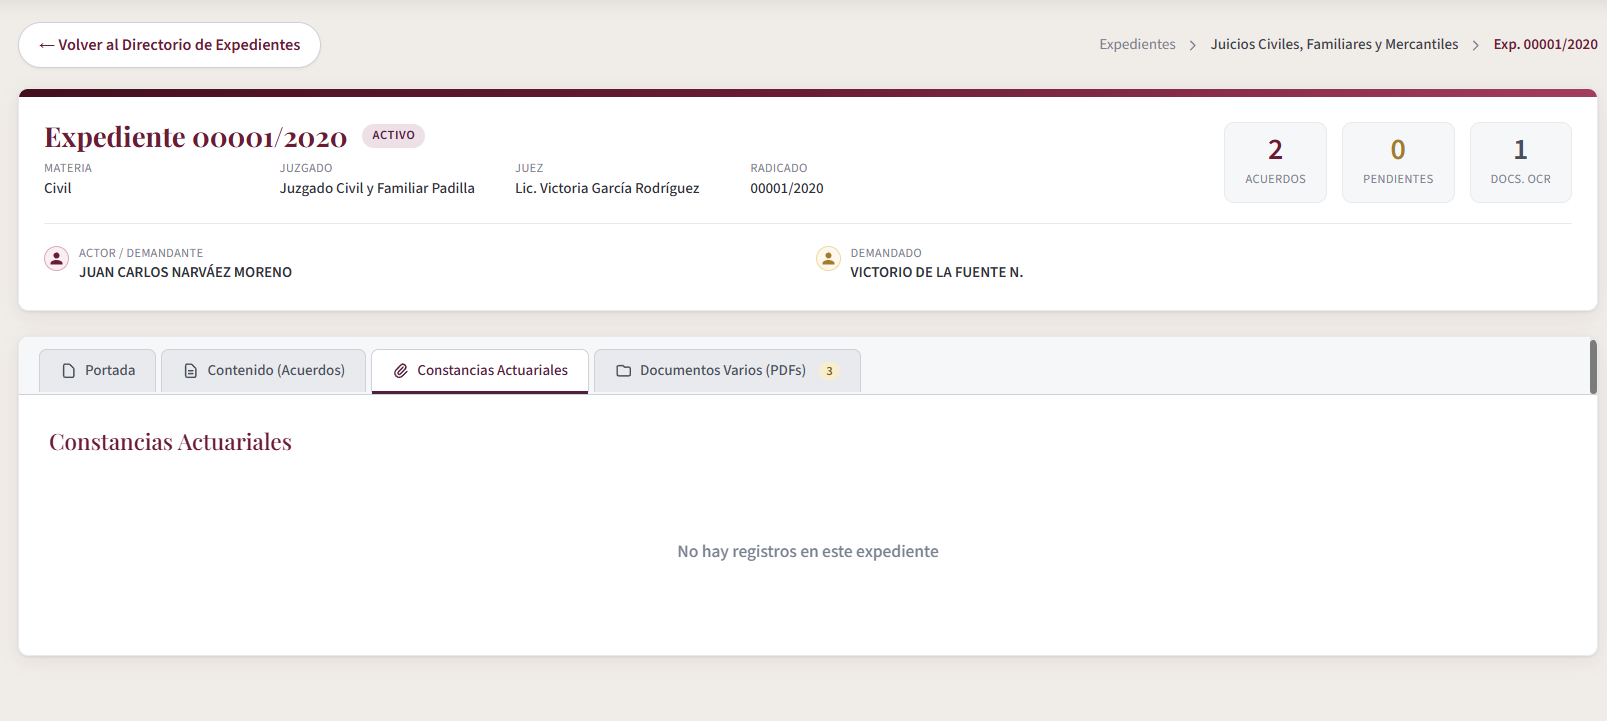
\includegraphics[width=0.9\textwidth]{img/Constancias.png}
    \caption{Pestaña para el control de constancias actuariales.}
    \label{fig:pantalla_constancias}
\end{figure}

\subsubsection{Carga de Promociones (Documentos Físicos)}
El proceso de automatización arranca cuando un abogado presenta un escrito (promoción). El personal del juzgado escanea el documento y se dirige a la pestaña \textbf{Documentos Varios (PDFs)}. Aquí, el sistema permite abrir el explorador de archivos de la computadora (Figura \ref{fig:pantalla_seleccionar}) para cargar el PDF. Una vez subido, el documento queda listado en pantalla con la opción habilitada para procesarlo (Figura \ref{fig:pantalla_documentos}).

\begin{figure}[H]
    \centering
    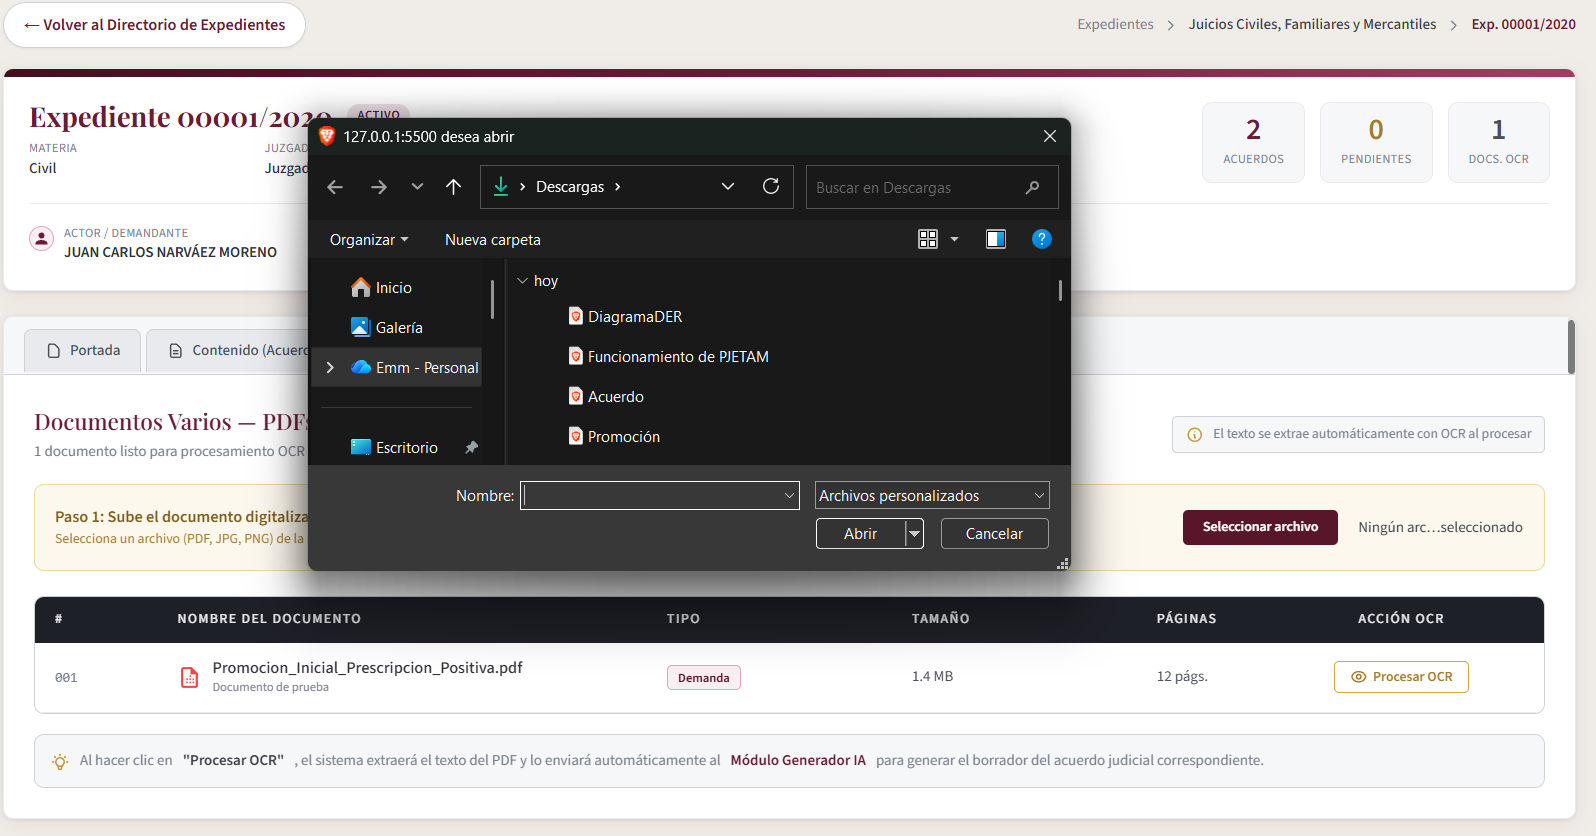
\includegraphics[width=0.85\textwidth]{img/Seleccionar_archivo.png}
    \caption{Selección del documento escaneado desde el equipo local.}
    \label{fig:pantalla_seleccionar}
\end{figure}

\begin{figure}[H]
    \centering
    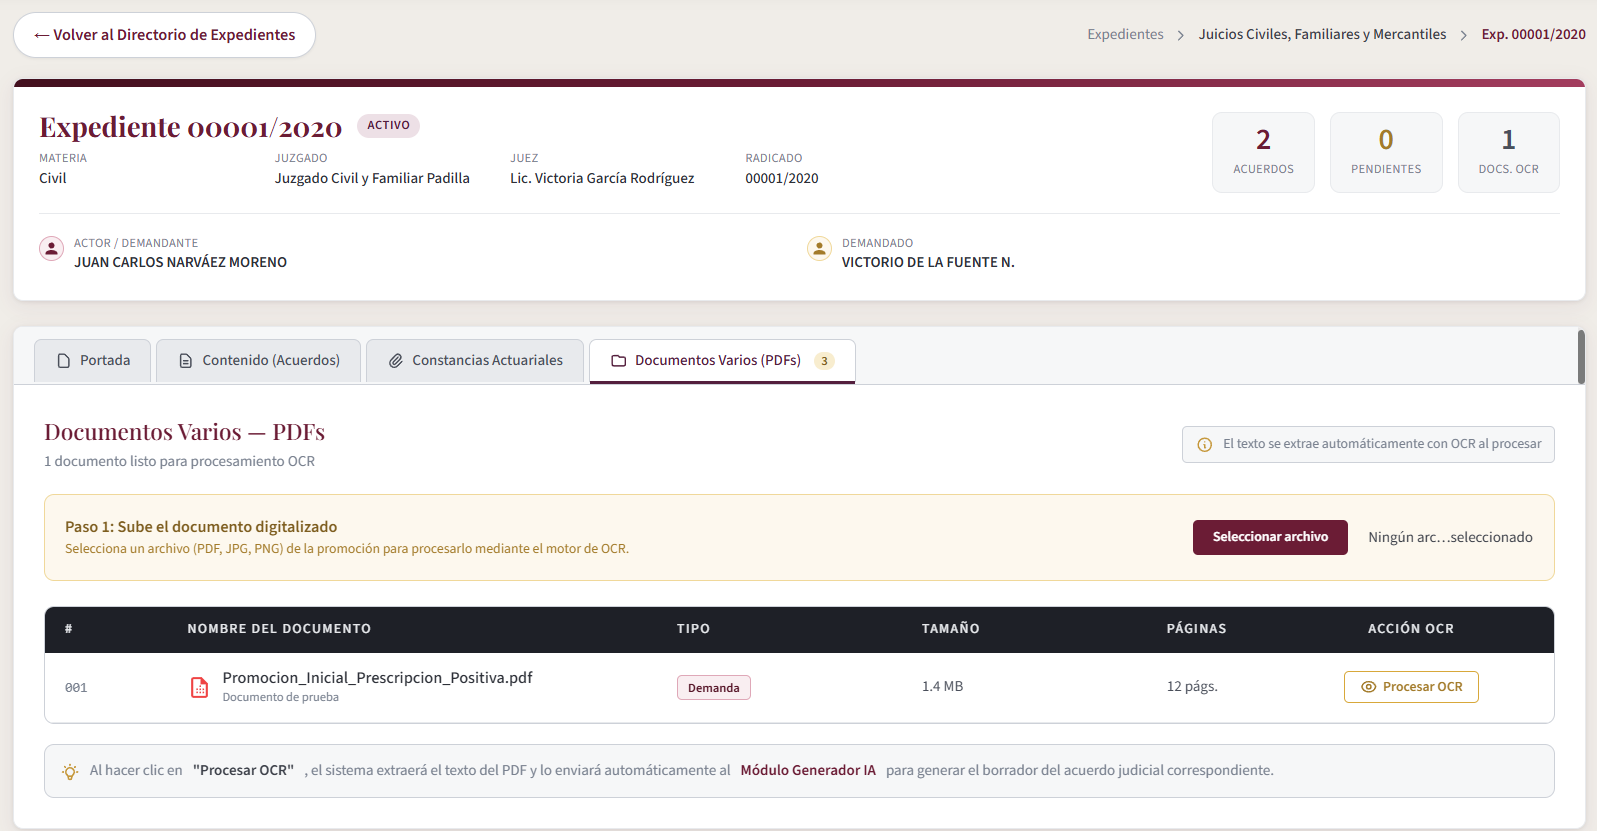
\includegraphics[width=0.9\textwidth]{img/Documento_varios.png}
    \caption{Documento cargado en el sistema, listo para extracción de texto.}
    \label{fig:pantalla_documentos}
\end{figure}

\subsubsection{Generación y Aprobación de Acuerdos con IA}
Al hacer clic en "Procesar OCR", el sistema entra en acción. Extrae el texto de la imagen del PDF y lo envía a la Inteligencia Artificial. El resultado se muestra en el módulo \textbf{Generador IA} (Figura \ref{fig:pantalla_generador}), el cual tiene una pantalla dividida:
\begin{itemize}
    \item \textbf{Lado izquierdo (Insumo):} Muestra el texto "crudo" que la máquina logró leer del PDF original.
    \item \textbf{Lado derecho (Salida):} Presenta un editor de texto avanzado que contiene la propuesta del acuerdo redactada por la IA, incluyendo los fundamentos legales citados (artículos del Código de Procedimientos Civiles).
\end{itemize}

\begin{figure}[H]
    \centering
    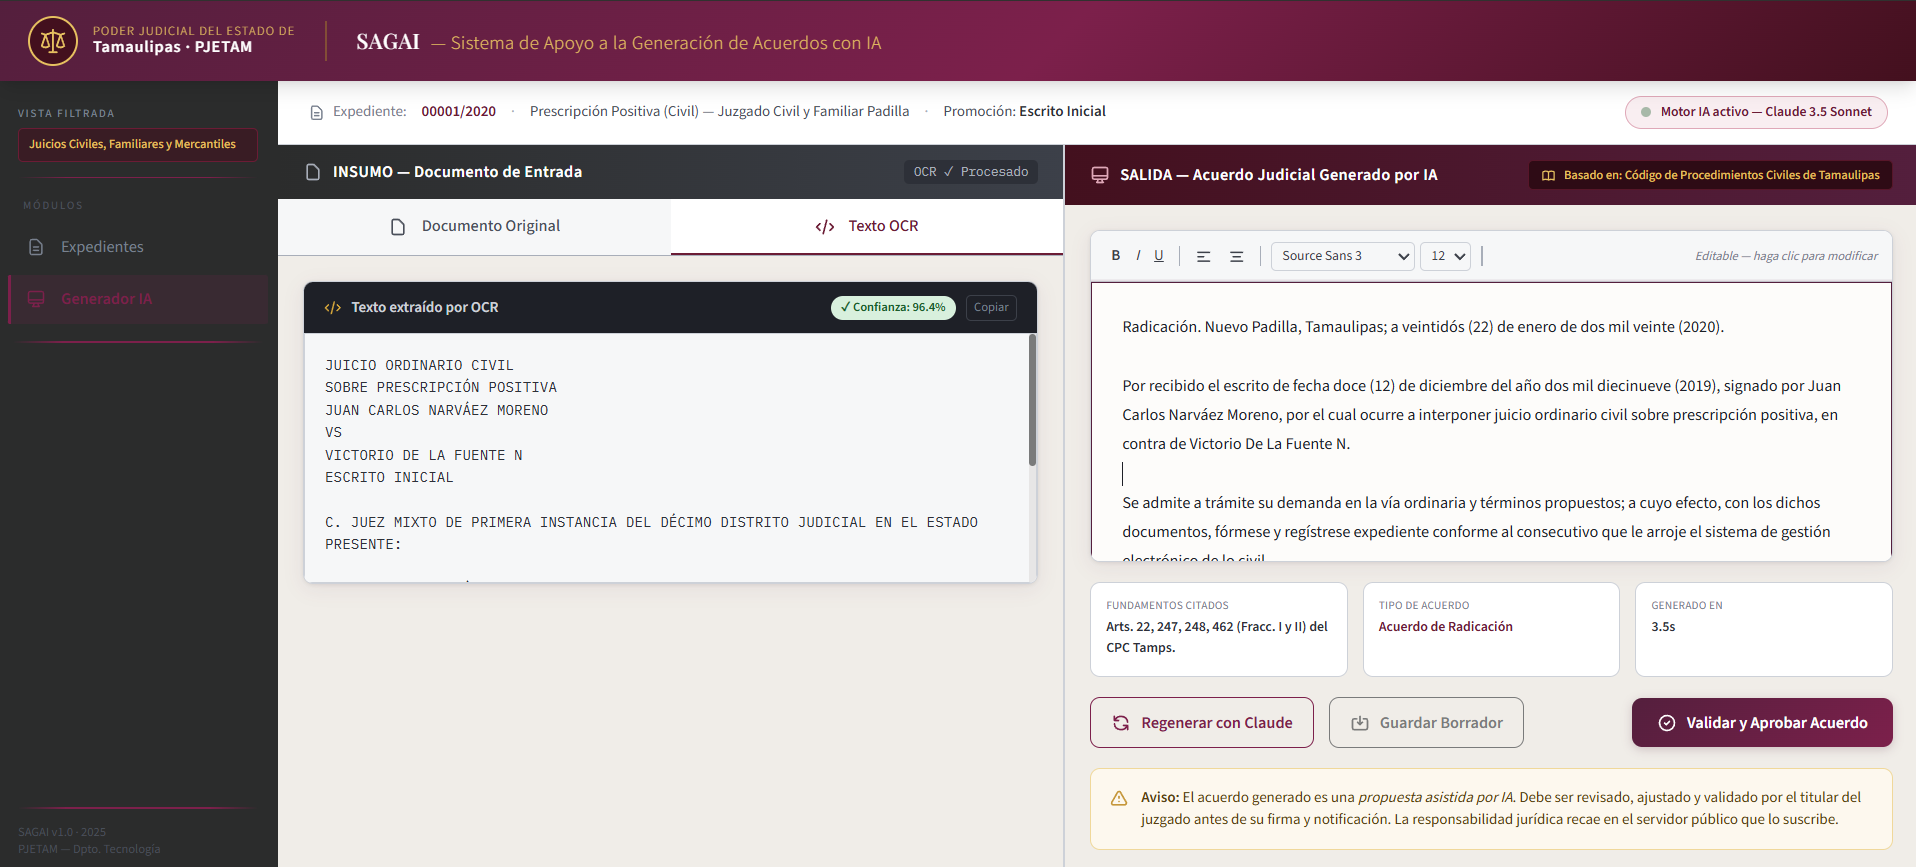
\includegraphics[width=0.9\textwidth]{img/Generador_ia.png}
    \caption{Pantalla dividida: Texto extraído (izq.) y borrador generado por la IA (der.).}
    \label{fig:pantalla_generador}
\end{figure}

Es vital destacar que el sistema está diseñado como una herramienta de apoyo, no de reemplazo. El usuario debe leer la propuesta, hacer correcciones si lo considera necesario en el editor derecho y, finalmente, dar su visto bueno. Al presionar "Validar y Aprobar Acuerdo", el sistema confirma el éxito de la operación (Figura \ref{fig:pantalla_aprobado}), guardando el documento oficialmente en la base de datos del expediente.

\begin{figure}[H]
    \centering
    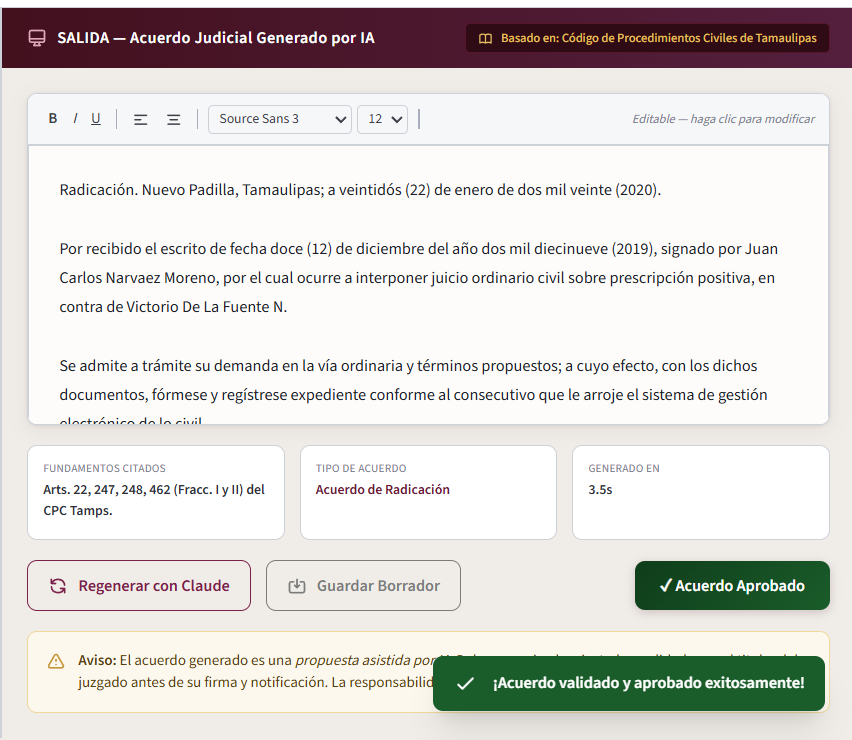
\includegraphics[width=0.7\textwidth]{img/Aprovado.png}
    \caption{Mensaje de éxito tras la validación y guardado del acuerdo final.}
    \label{fig:pantalla_aprobado}
\end{figure}